\documentclass{standalone}

\begin{document}

\subsection{SARSA}


\begin{figure}[H]
	\center
	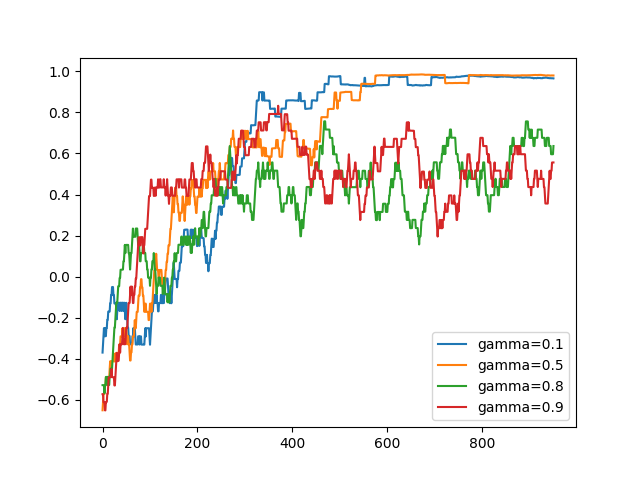
\includegraphics[scale=0.7]{img/sarsa.png}
	\caption{Algorithme Sarsa}
	\label{ql:sarsa}
\end{figure}

\subsection{Dyna Q}

\begin{minted}{python}
    def updateQ(self, st, at, rt, stp, alpha=0.9, gamma=0.9, alphar=0.8):

        st = self.state_dict[st.dumps()]
        stp = self.state_dict[stp.dumps()]
        self.Q[st, at] = (1 - alpha) * self.Q[st, at] + alpha * (rt + gamma * np.max(self.Q[stp, :]))

        self.R[st, at, stp] = (1 - alphar) * self.R[st, at, stp] + alphar * rt
        self.P[stp, st, at] = (1 - alphar) * self.P[stp, st, at] + alphar

        for s in range(max(self.states) + 1):
            if s != stp:
                self.P[s, st, at] = (1 - alphar) * self.P[s, st, at]

        self.P = softmax(self.P)

        states = list(self.state_dict.values())

        s = list(np.random.choice(states, self.k))
        a = list(np.random.choice(self.actions, self.k))

        for i in range(self.k):
            self.Q[s[i], a[i]] = (1 - alpha) * self.Q[s[i], a[i]] + alpha * \
                                 (sum([self.P[sp, s[i], a[i]] * (self.R[s[i], a[i], sp] +
                                                                 gamma * np.max(self.Q[sp, :]))
                                       for sp in s]))

\end{minted}


\begin{figure}[!ht]
	\center
	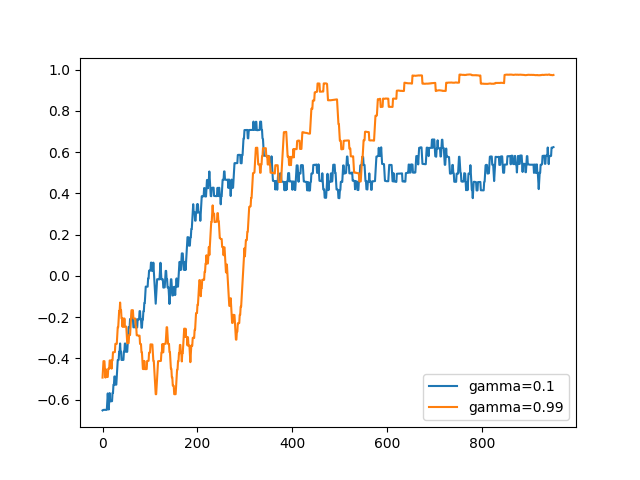
\includegraphics[scale=0.7]{img/dynaq.png}
	\caption{Algorithme DynaQ}
	\label{ql:dynaq}
\end{figure}





\end{document}
